\documentclass[aspectratio=169,11pt,hyperref={colorlinks=true}]{beamer}
\usepackage[utf8]{inputenc}
\usepackage[T1]{fontenc}
\usepackage{fontspec}
\usepackage[absolute,overlay]{textpos}
\usepackage{listingsutf8}
\usepackage{listings-golang}
\usepackage{tikz}
\usepackage{color}


\title{Tekton 101}
\date[kubeconna2019]{November 19th 2019}
\author[Andrea]{%
  Andrea Frittoli \\
  Open Source Developer Advocate \\
  andrea.frittoli@uk.ibm.com \\
  @blackchip76
}
\institute[kubeconna2019]{%
  KubeCon and CloudNativeCon North America 2019
}

\usetheme{ibmcloud}

% Code style
\setlststyle

\lstdefinelanguage{koyaml}{
  keywords={github, com, afrittoli, examples, ms, go, helloworld},
  sensitive=false,
  comment=[l]{\#},
  morestring=[b]',
  morestring=[b]"
}

% Automatic section frame
\AtBeginSection{\frame{\sectionpage}}

\begin{document}

\begin{frame}[noframenumbering]
\titlepage{}
\end{frame}

% The main points of the talk are (TBD):
% - Give an introduction to Tekton Pipelines
% - Get in some more details with an example
% - Talk about Kaniko and source to image with tricky bits
% - Reusing tasks, dev vs CI vs CD
% - can I use Tekton? Where? security concerns

% The slide/section order does not match the narrative yet

%% TBD

\section{A Bit of History}

\begin{lblackrwhiteframe}
  \frametitle{Knative Build}
  \large
  \begin{beamercolorbox}[wd=0.4\paperwidth]{text}
    \begin{itemize}
      \item Beginning of 2018...
      \item Knative:
      \begin{itemize}
        \item Build
        \item Eventing
        \item Serving
      \end{itemize}
      \item Sept 2018...
      \item Knative Pipelines
    \end{itemize}
    \begin{itemize}
      \item OpenSource
      \item Contributors:
      \begin{itemize}
        \item[] Google, RedHat, IBM
        \item[] Cloudbees, Pivotal
        \item[] ...and others
      \end{itemize}
    \end{itemize}
  \end{beamercolorbox}%
  \begin{textblock*}{0.5\paperwidth}(0.5\paperwidth,0.2\paperheight)
    \centering
    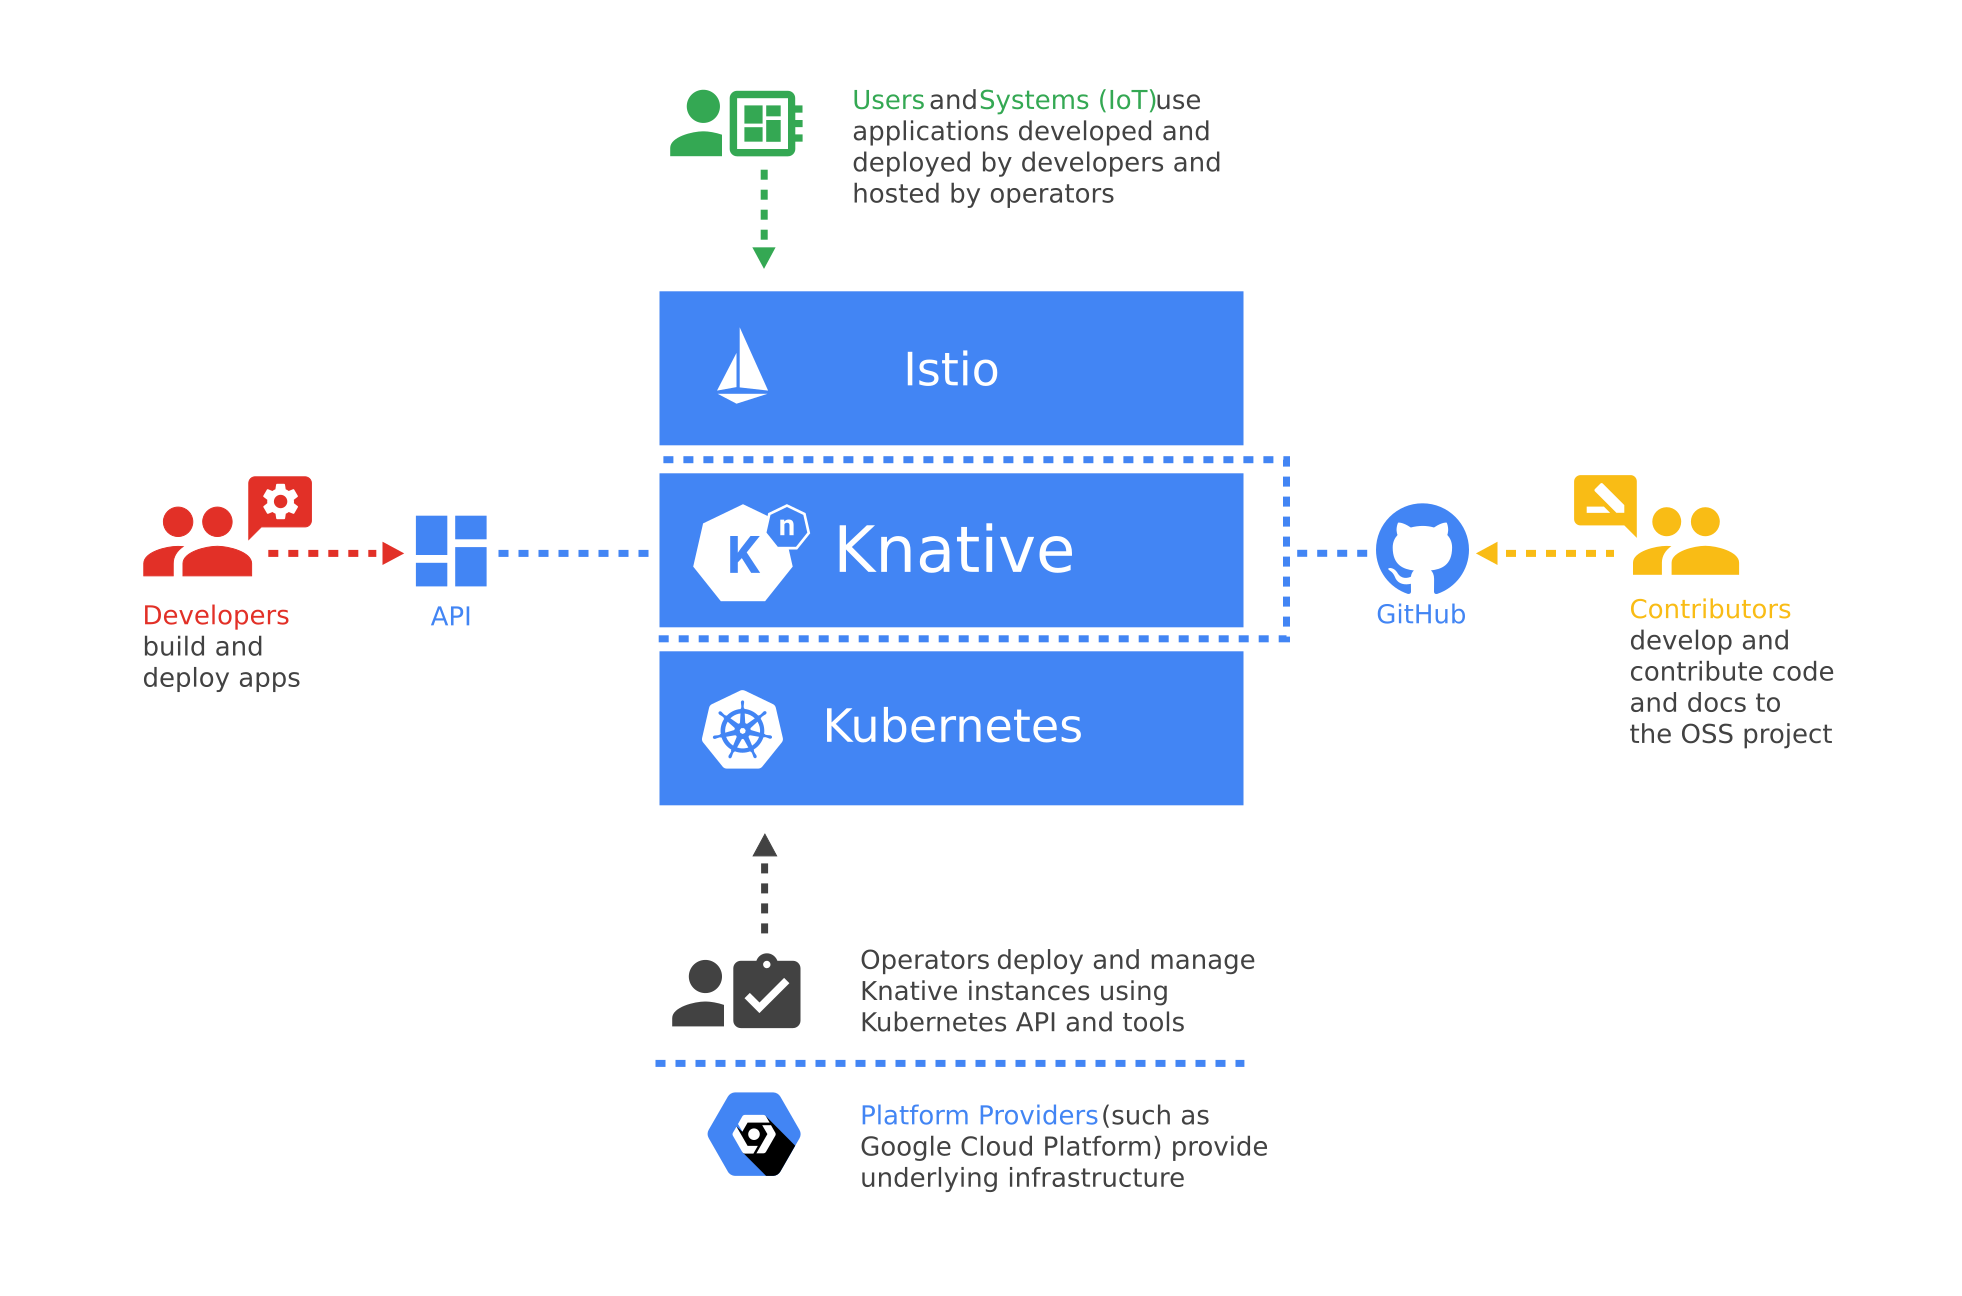
\includegraphics[width=0.45\paperwidth]{img/knative-audience.png}
  \end{textblock*}
\end{grayframe}

\begin{lwhiterblackframe}
  \frametitle{From Knative to Tekton}
  \large
  \begin{textblock*}{0.5\paperwidth}(0.5\paperwidth,0.25\paperheight)
    \centering
    
\includegraphics[width=0.35\paperwidth]{img/tekton-horizontal-color.png}
    
\includegraphics[width=0.20\paperwidth]{img/cdf-color.png}
  \end{textblock*}
  \begin{beamercolorbox}[wd=0.35\paperwidth]{text}
    \begin{itemize}
      \item Tekton pipelines (March 2019)
      \item Focus on CI/CD
      \item @CD Foundation  (March 2019)
      \item Deploy ``anywhere''
      \item Replaces Knative Build (June 2019)
      \item Bootstrap governance
      \item Build deprecated in Knative
    \end{itemize}
  \end{beamercolorbox}%
\end{lblackrwhiteframe}

% \begin{blackframe}
%   \frametitle{\textasciitilde Sept 2018: Knative Pipelines}
%   \begin{textblock*}{\paperwidth}(0cm,0.2\paperheight)
%     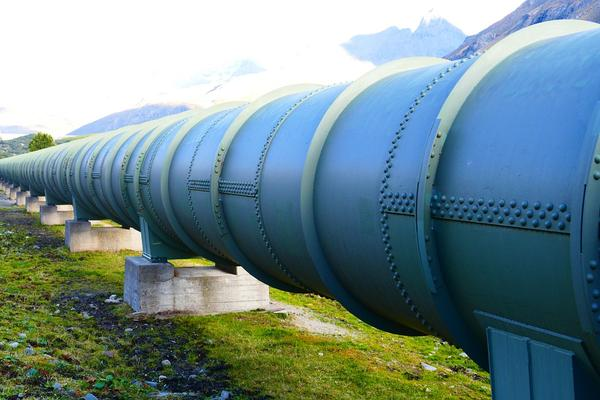
\includegraphics[width=\paperwidth]{img/pipeline_cc0.jpg}
%     % https://mediad.publicbroadcasting.net/p/shared/npr/styles/placed_wide/nprshared/201804/605180710.jpg
%   \end{textblock*}
%   \begin{textblock*}{0.2\paperwidth}(0.83\paperwidth,0.93\paperheight)
%     
\includegraphics[width=0.03\paperwidth]{img/cc.png}
%     
\includegraphics[width=0.03\paperwidth]{img/zero.png}
%   \end{textblock*}
% \end{blackframe}

\section{Tekton Pipelines}

\begin{fullscreenslide}
{img/overview.png}
\end{fullscreenslide}


\begin{blackframe}
  \frametitle{Cloud Native Pipelines}
  % Cloud Native Pipelines, run on Kubernetes
  \begin{textblock*}{\paperwidth}(0.05\paperwidth,0.2\paperheight)
    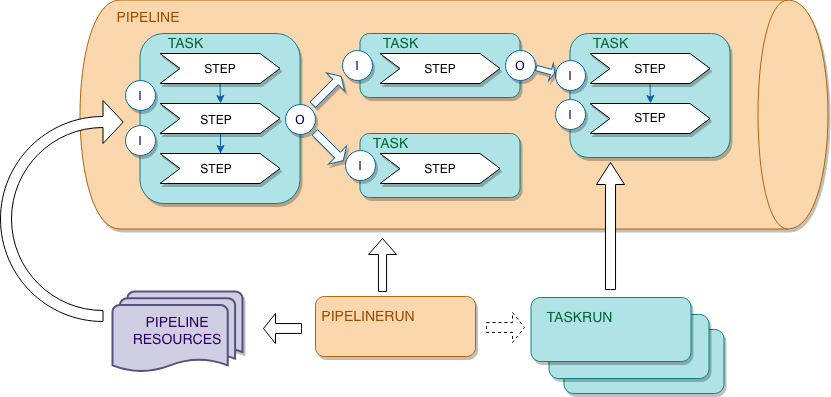
\includegraphics[width=0.85\paperwidth]{img/tekton.png}
  \end{textblock*}
  \begin{textblock*}{0.2\paperwidth}(0.9\paperwidth,0.83\paperheight)
    
\includegraphics[width=0.03\paperwidth]{img/cc.png}
    
\includegraphics[width=0.03\paperwidth]{img/zero.png}
  \end{textblock*}
\end{grayframe}

\begin{2columnsframe}
  {
    \begin{itemize}
      \item Steps are sequential
      \item Tasks are a Directed Acyclic Graph
      \item Order defined by:
      \begin{itemize}
        \item {\em from}: input / output
        \item {\em runAfter}: enforced ordering
      \end{itemize}
    \end{itemize}
  }
  % Graph of a CD pipeline
  {
  \begin{textblock*}{0.65\paperwidth}(0.30\paperwidth,0.30\paperheight)
    \centering
    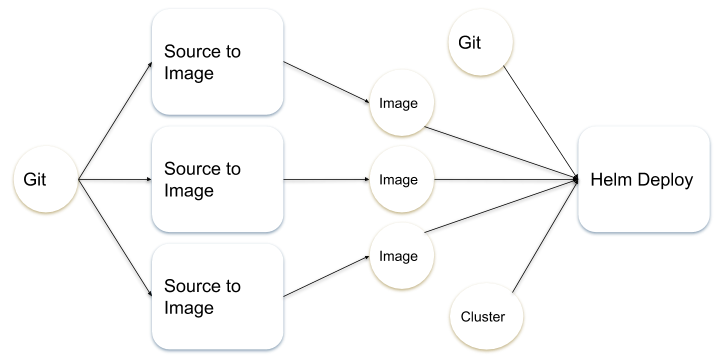
\includegraphics[width=0.65\paperwidth]{img/pipeline.png}
  \end{textblock*}
  }
  \frametitle{Sample pipeline}
\end{2columnsframe}

% \begin{2columnsframe}
%   {
%   {\tiny Source to Image (spec only): \\}
%   \lstinputlisting[language=koyaml,firstline=6,lastline=31]{code/task-source-to-image.yaml}
%   }
%   {
%   \lstinputlisting[language=koyaml,firstline=32,lastline=55]{code/task-source-to-image.yaml}
%   % {\tiny Cache Warmer (spec only): \\}
%   % \lstinputlisting[language=koyaml,firstline=21,lastline=35]{code/task-kaniko-cache.yaml}
%   }
%   \frametitle{Sample Task: Source to Image}
% \end{2columnsframe}

% \begin{2columnsframe}
%   {
%   \begin{itemize}
%     \item Pipeline and Tasks:
%     \begin{itemize}
%       \item Static definition, stored in git
%     \end{itemize}
%     \item PipelineRuns and TaskRuns:
%     \begin{itemize}
%       \item Specific to one execution
%       \item Generated programmatically
%     \end{itemize}
%     \item Parameters and Resources:
%     \begin{itemize}
%       \item Env / run specific
%     \end{itemize}
%   \end{itemize}
%   \vspace{0.3ex}
%   \lstinputlisting[language=koyaml]{code/resource-git.yaml}
%   }
%   {
%   \lstinputlisting[language=koyaml]{code/resource-cluster.yaml}
%   \vspace{0.3ex}
%   \lstinputlisting[language=koyaml]{code/resource-image.yaml}
%   }
%   \frametitle{Pipeline as code}
% \end{2columnsframe}

\section{Tekton Projects}

\begin{2columnsmoreleftframe}
  {
  \begin{itemize}
    \item tektoncd/pipeline — core
    \item tektoncd/catalog — shareable task definition
    \item tektoncd/cli — command-line to interact with pipeline
    \item tektoncd/triggers — create tekton resources in reaction of events
    \item tektoncd/operator — install/upgrade you tekton
    \item tektoncd/dashboard — web ui for tekton
    \item[]
    \item Plumbing, Community, Website (https://tekton.dev/), Friends
  \end{itemize}
  }
  {
  % \begin{itemize}
  %   \item Plumbing
  %   \item Community
  %   \item Friends
  %   \item Website (https://tekton.dev/)
  % \end{itemize}
  \begin{textblock*}{0.25\paperwidth}(0.70\paperwidth,0.40\paperheight)
    \centering
    
\includegraphics[width=0.25\paperwidth]{img/tekton-friends.png}
  \end{textblock*}
  }
  \frametitle{Tekton projects}
\end{2columnsmoreleftframe}

\begin{centraldark}{Thank You!}\end{centraldark}

\begin{grayframe}
  \frametitle{References}
  \begin{itemize}
    \item This Talk: https://github.com/afrittoli//github.com/afrittoli/tekton101/tree/kubecon-na-2019
    \item Tekton Links:
    \begin{itemize}
      \item https://tekton.dev/, https://cd.foundation/
      \item https://github.com/tektoncd/pipeline
      \item https://github.com/tektoncd/pipeline/blob/master/roadmap-2019.md
    \end{itemize}
    \item IBM Cloud: https://cloud.ibm.com
  \end{itemize}
\end{grayframe}

\section{Q\&A}

\end{document}
